\begin{figure}[htbp]
  \centering
  \definecolor{vtYieldBg}{HTML}{EEF7F2}
  \definecolor{vtYieldEdge}{HTML}{1F6F50}
  \definecolor{vtPinBg}{HTML}{FFF6E6}
  \definecolor{vtPinEdge}{HTML}{B45309}
  \definecolor{vtJniBg}{HTML}{FDECEC}
  \definecolor{vtJniEdge}{HTML}{991B1B}
  \definecolor{vtNeutralBg}{HTML}{F4F6F8}
  \definecolor{vtNeutralEdge}{HTML}{475569}

  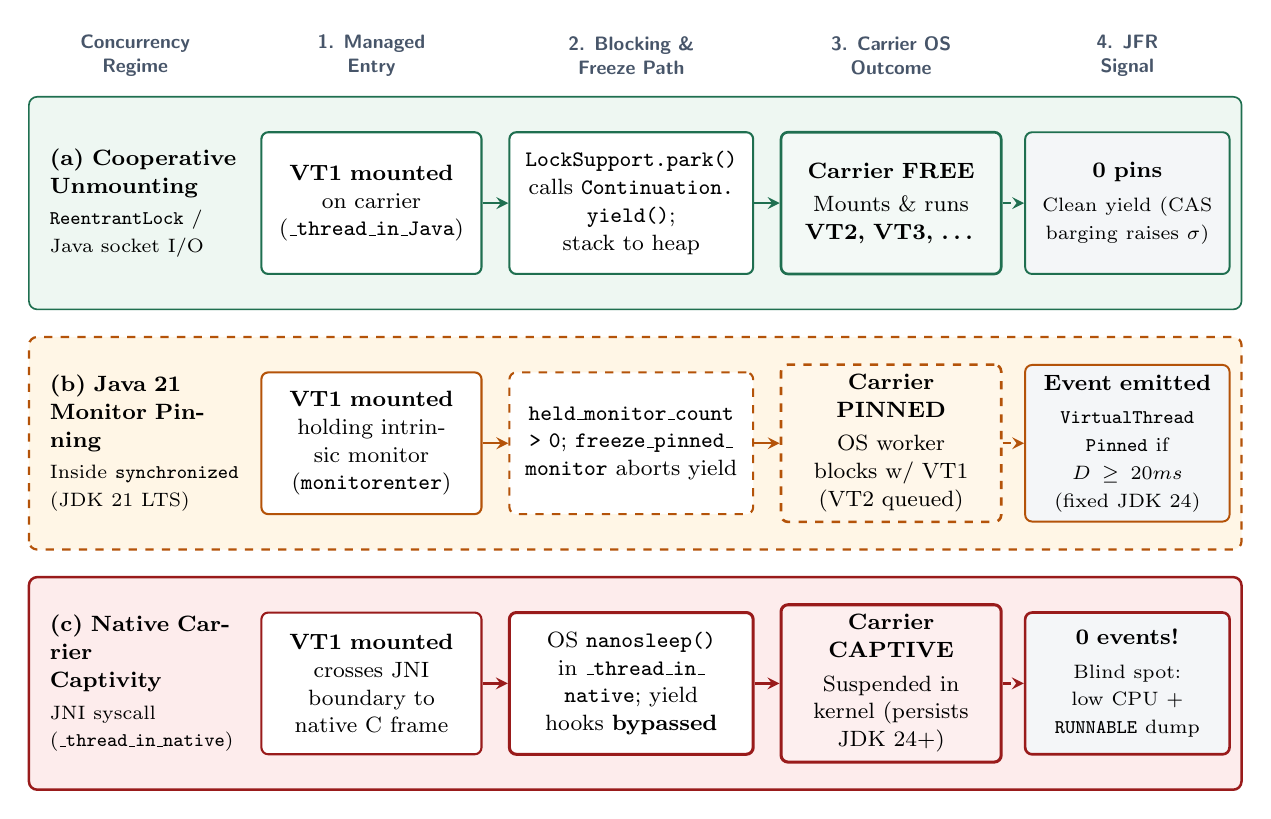
\begin{tikzpicture}[
      x=1cm, y=1cm, >=stealth,
      node font=\footnotesize\linespread{1.06}\selectfont,
      stagebox/.style={rounded corners=2.5pt, draw=#1, fill=white, line width=0.75pt,
                       minimum height=1.80cm, text width=2.55cm, align=center, inner sep=3.5pt},
      widebox/.style={rounded corners=2.5pt, draw=#1, fill=white, line width=0.75pt,
                      minimum height=1.80cm, text width=2.85cm, align=center, inner sep=3.5pt},
      outcomebox/.style 2 args={rounded corners=2.5pt, draw=#1, fill=#2, line width=0.95pt,
                         minimum height=1.80cm, text width=2.55cm, align=center, inner sep=3.5pt},
      jfrbox/.style={rounded corners=2.5pt, draw=vtNeutralEdge, fill=vtNeutralBg, line width=0.7pt,
                     minimum height=1.80cm, text width=2.35cm, align=center, inner sep=3.5pt},
      hdr/.style={font=\scriptsize\bfseries\sffamily, text=vtNeutralEdge, align=center},
      flow/.style={->, line width=0.9pt, draw=vtNeutralEdge}
    ]

    % Column Headers (two-line clean labels, zero collisions)
    \node[hdr] at (1.35, 9.52) {Concurrency\\Regime};
    \node[hdr] at (4.35, 9.52) {1. Managed\\Entry};
    \node[hdr] at (7.65, 9.52) {2. Blocking \&\\Freeze Path};
    \node[hdr] at (10.95, 9.52) {3. Carrier OS\\Outcome};
    \node[hdr] at (13.95, 9.52) {4. JFR\\Signal};

    % -------------------------------------------------------------------------
    % Row (a): Cooperative Unmounting
    % -------------------------------------------------------------------------
    \fill[vtYieldBg, rounded corners=3pt] (0, 6.30) rectangle (15.40, 9.00);
    \draw[vtYieldEdge, line width=0.6pt, rounded corners=3pt] (0, 6.30) rectangle (15.40, 9.00);

    \node[text width=2.40cm, align=left, anchor=west] at (0.16, 7.65) {%
      {\bfseries (a) Cooperative\\Unmounting}\\[3pt]
      \scriptsize \texttt{ReentrantLock} /\\Java socket I/O%
    };

    \node[stagebox=vtYieldEdge] (a1) at (4.35, 7.65) {%
      \textbf{VT1 mounted} on carrier\\(\texttt{\_thread\_\allowbreak in\_Java})%
    };
    \node[widebox=vtYieldEdge] (a2) at (7.65, 7.65) {%
      \texttt{LockSupport.\allowbreak park()} calls \texttt{Continuation.\allowbreak yield()}; stack to heap%
    };
    \node[outcomebox={vtYieldEdge}{vtYieldBg!70!white}] (a3) at (10.95, 7.65) {%
      \textbf{Carrier FREE}\\[2pt]
      Mounts \& runs\\ \textbf{VT2, VT3, \dots}%
    };
    \node[jfrbox, draw=vtYieldEdge] (a4) at (13.95, 7.65) {%
      \textbf{0 pins}\\[2pt]
      \scriptsize Clean yield (CAS barging raises $\sigma$)%
    };

    \draw[flow, draw=vtYieldEdge] (a1) -- (a2);
    \draw[flow, draw=vtYieldEdge] (a2) -- (a3);
    \draw[flow, draw=vtYieldEdge, dashed] (a3) -- (a4);

    % -------------------------------------------------------------------------
    % Row (b): Java 21 Monitor Pinning
    % -------------------------------------------------------------------------
    \fill[vtPinBg, rounded corners=3pt] (0, 3.25) rectangle (15.40, 5.95);
    \draw[vtPinEdge, dashed, line width=0.8pt, rounded corners=3pt] (0, 3.25) rectangle (15.40, 5.95);

    \node[text width=2.40cm, align=left, anchor=west] at (0.16, 4.60) {%
      {\bfseries (b) Java~21\\Monitor Pinning}\\[3pt]
      \scriptsize Inside \texttt{synchronized}\\(JDK~21 LTS)%
    };

    \node[stagebox=vtPinEdge] (b1) at (4.35, 4.60) {%
      \textbf{VT1 mounted} holding intrinsic monitor (\texttt{monitorenter})%
    };
    \node[widebox=vtPinEdge, dashed] (b2) at (7.65, 4.60) {%
      \texttt{held\_monitor\_\allowbreak count > 0}; \texttt{freeze\_pinned\_\allowbreak monitor} aborts yield%
    };
    \node[outcomebox={vtPinEdge}{vtPinBg!85!white}, dashed] (b3) at (10.95, 4.60) {%
      \textbf{Carrier PINNED}\\[2pt]
      OS worker blocks w/ VT1 (VT2 queued)%
    };
    \node[jfrbox, draw=vtPinEdge] (b4) at (13.95, 4.60) {%
      \textbf{Event emitted}\\[2pt]
      \scriptsize \texttt{VirtualThread\-\allowbreak Pinned} if $D \ge 20\text{ ms}$ (fixed JDK~24)%
    };

    \draw[flow, draw=vtPinEdge] (b1) -- (b2);
    \draw[flow, draw=vtPinEdge] (b2) -- (b3);
    \draw[flow, draw=vtPinEdge, dashed] (b3) -- (b4);

    % -------------------------------------------------------------------------
    % Row (c): Native Carrier Captivity (JNI)
    % -------------------------------------------------------------------------
    \fill[vtJniBg, rounded corners=3pt] (0, 0.20) rectangle (15.40, 2.90);
    \draw[vtJniEdge, line width=0.9pt, rounded corners=3pt] (0, 0.20) rectangle (15.40, 2.90);

    \node[text width=2.40cm, align=left, anchor=west] at (0.16, 1.55) {%
      {\bfseries (c) Native Carrier\\Captivity}\\[3pt]
      \scriptsize JNI syscall\\(\texttt{\_thread\_\allowbreak in\_native})%
    };

    \node[stagebox=vtJniEdge] (c1) at (4.35, 1.55) {%
      \textbf{VT1 mounted} crosses JNI boundary to native C frame%
    };
    \node[widebox=vtJniEdge, line width=1.1pt] (c2) at (7.65, 1.55) {%
      OS \texttt{nanosleep()} in \texttt{\_thread\_in\_\allowbreak native}; yield hooks \textbf{bypassed}%
    };
    \node[outcomebox={vtJniEdge}{vtJniBg!85!white}, line width=1.1pt] (c3) at (10.95, 1.55) {%
      \textbf{Carrier CAPTIVE}\\[2pt]
      Suspended in kernel (persists JDK~24+)%
    };
    \node[jfrbox, draw=vtJniEdge, line width=0.95pt] (c4) at (13.95, 1.55) {%
      \textbf{0 events!}\\[2pt]
      \scriptsize Blind spot: low CPU + \texttt{RUNNABLE} dump%
    };

    \draw[flow, draw=vtJniEdge] (c1) -- (c2);
    \draw[flow, draw=vtJniEdge] (c2) -- (c3);
    \draw[flow, draw=vtJniEdge, dashed] (c3) -- (c4);
  \end{tikzpicture}
  \caption[HotSpot Virtual Thread carrier unmounting, Java~21 monitor pinning, and native JNI captivity.]{HotSpot Virtual Thread carrier scheduling paths on Java~21: (a)~cooperative unmounting onto the heap under AQS/socket I/O, (b)~monitored \texttt{synchronized} pinning returning \texttt{freeze\_pinned\_monitor} with JFR threshold emission ($\ge 20\text{ ms}$), and (c)~JNI \texttt{\_thread\_in\_native} carrier captivity that bypasses continuation yield hooks and emits zero JFR pinning events.}
  \label{fig:carrier-lifecycle}
\end{figure}
